% Netzwerkanltung für die Studentenstadt Freimann
% Tex initially created by Maximilian Engelhardt <maximilian.engelhardt@stusta.mhn.de>

%\documentclass[a4paper,12pt,draft]{scrartcl}
\documentclass[a4paper,12pt]{scrartcl}

\usepackage[utf8]{inputenc}
\usepackage{ngerman}
\usepackage{eurosym}
\usepackage{tabularx}
%\usepackage[T1]{fontspec}
%\usepackage{newcomputermodern}
\renewcommand*{\familydefault}{\sfdefault}
\usepackage[pdftex,final]{graphicx}
\usepackage[top=1.5cm,bottom=2.5cm,left=1.5cm,right=1.5cm]{geometry}
%\usepackage[margin=2cm]{geometry}
%\usepackage{hyperref}
\usepackage[hidelinks]{hyperref}
\usepackage{booktabs}

\title{Wohnanlage Studentenstadt Freimann:\\
       Anleitung zum Einrichten des Internetzugangs}
%\date{\today}

\begin{document}

\maketitle

\begin{figure}[t!]
   \centering
   \vspace{-20pt}
   
\includegraphics[width=0.8\textwidth,keepaspectratio]{Bilder/StuStaNet_Logo}
   \vspace{-40pt}
\end{figure}

\tableofcontents
\newpage

\section{Allgemeine Informationen zum Netzwerkanschluss}
Es gibt kein von uns gestelltes WLAN-Netz in den Zimmern, deshalb ist es notwendig, den Netzwerkzugang selbst einzurichten.
Somit kann jeder für WLAN selber einen Access Point z.B. mithilfe eines Routers betreiben.

Es gibt zwei Möglichkeiten das Internet zu benutzen, die in dieser Anleitung erklärt werden.
Ohne Mitgliedschaft ist der Zugang nur über unseren Proxyserver möglich.
Dieser muss in jedem Programm eingestellt und auch davon unterstützt werden.
Bei einiger Software funktioniert die manuelle Proxyeinrichtung nicht, wie beispielsweise bei WhatsApp oder League of Legends.

Das erlaubt die zweite Option, eine Mitgliedschaft beim StuStaNet~e.\,V.\@

\section{Mitgliedschaft StuStaNet~e.\,V.\@}
Als Mitglied erfolgt der Zugang über unser NAT-Gateway.
Die Konfiguration des Proxys auf den Geräten kann damit entfallen.
Außerdem stehen für Mitglieder des StuStaNet weitere nützliche Dienste (\url{https://wiki.stusta.de/Dienste}) wie eine eigene E-Mail-Adresse, Webspace, ein Backupserver oder WLAN in einigen Gemeinschaftseinrichtungen der StuSta (\url{https://stustanet.de/de/wifi/}) zur Verfügung. 

Für die Mitgliedschaft fällt eine einmalige Aufnahmegebühr von derzeit \EUR{20} an.
Zurzeit gibt es zudem keinen regelmäßigen Mitgliedsbeitrag.
Um Mitglied zu werden, musst man sich auf \mbox{\url{https://reg.stustanet.de}} registrieren und danach den unterschriebenen Mitgliedsantrag in unseren Briefkasten (\textit{StuStaNet~e.\,V.\@} in Haus 10) einwerfen.
Alternativ kann die Anmeldung auch in der Sprechstunde stattfinden.
Diese findet regelmäßig in Haus 10, Zimmer 002 (Kellergeschoss) donnerstags 19:00-19:30 Uhr statt.
Der aktuelle Terminplan ist unter \mbox{\url{https://stustanet.de}} einsehbar.

Die Adresse von Haus 10 lautet: Hans-Leipelt-Straße 7, 80805 München.

\section{Allgemeine Informationen zur Einrichtung}
\label{sec:general}

\subsection{Zettel mit IP-Adressen des Zimmers}
\label{ip_sheet}
\begin{minipage}{0.57\textwidth}
Für die Einrichtung wird der Zettel mit den IP-Adressen des Zimmers benötigt.
Dieser wird beim Einzug ausgehändigt oder als Anhang zu der Mail mit den Vertragsunterlagen versendet.
Die jeweilige IP-Adresse steht auch auf dem Aufkleber auf der Netzwerkdose im Zimmer.
Sollte beides nicht auffindbar sein, kann der Servicedesk des Studentenwerks weiterhelfen.

Wichtig ist dabei, dass die \textbf{Netzmaske} auf dem Zettel dabei der \textbf{Subnetzmaske} in manchen Betriebssystemen entspricht und die entsprechende \textbf{Subnetzpräfixlänge} 24 beträgt.
\end{minipage}
\hfill
\begin{minipage}{0.4\textwidth}
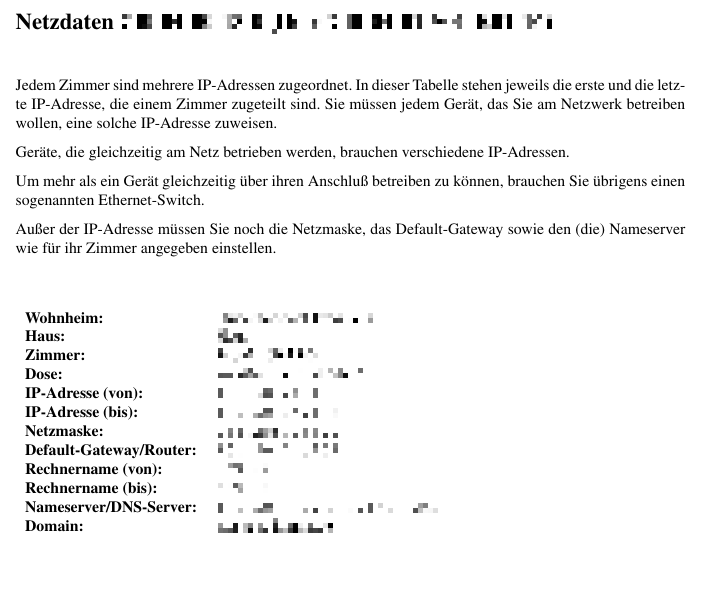
\includegraphics[width=\linewidth]{Bilder/ip_zettel}
%  \caption{Bildunterschrift}
\end{minipage}

\subsection{Verbinden eines Computers oder eines Routers mit der Netzwerkdose}
Ein Computer kann entweder direkt über ein LAN-Kabel mit der Netzwerkdose verbunden oder es kann ein Router angeschlossen werden.
Im Regelfall funktioniert dabei nur die \textbf{linke} Dose, die auch oft entsprechend markiert ist. 
Um auch WLAN verwenden zu können und für die Verwendung von mehreren Geräten ist langfristig die Nutzung eines Routers zu empfehlen.

LAN-Kabel und Router können im Handel oder als Mitglied auch beim StuStaNet während der Sprechstunde (siehe weiter unten) erworben werden.

\subsection{Proxy für Nicht-Mitglieder}

Falls man nicht Mitglied beim StuStaNet ist, muss für jedes Gerät das im Zimmer benutzt werden soll entweder das Proxyskript verwendet (empfohlen) oder manuell den Proxyserver einstellt werden.
Nicht alle Programme unterstützen dabei die globalen Proxy-Einstellungen des Betriebssystems und unter Umständen müssen diese auch für einzelne Programme separat eingestellt werden.

\subsection{Zusammenfassung
}
Das Einrichten der Internetanbindung besteht somit aus folgenden Teilen:
\begin{itemize}
	\item Anschluss des Routers oder Computers an die Netzwerkbuchse (im Regelfall der linke, entsprechend auch markierte, Stecker)
	\item \textbf{Kapitel~\ref{sec:network_address}}: Konfiguration der Netzwerkeinstellungen bzw.\@ IP-Adressen des Routers oder Computers (wenn ohne Router direkt an Buchse angeschlossen)
	\item \textbf{Kapitel~\ref{sec:proxy}}: \textit{Nur für Nicht-Mitglieder:} Eintragen des Proxyservers bzw. -skripts auf allen Geräten bzw. Programmen
\end{itemize}

Falls der Router mit den Netzwerkeinstellungen konfiguriert wurde, dürfen die IP-Adressen nicht auch auf dem Computer oder Smartphone eingestellt werden!

Bei Problemen gibt es eine kurze Hilfe in Kapitel~\ref{sec:debugging}.
\\
\\
\noindent\begin{minipage}{\textwidth}

\subsection{Übersicht Netzwerkeinstellungen mit den jeweiligen Proxy-Konfigurationen}
\label{subsec:settings}
Pro Anschluss stehen 8 IP-Adressen zur Verfügung, wovon jede benutzt werden kann.
Der jeweilige Adressbereich ist auf der Netzwerkdose vermerkt oder auf dem Zettel mit den IP-Adressen aus Punkt~\ref{ip_sheet} zu finden.

\begin{center}
  \begin{tabularx}{\linewidth}{lXp{.2\linewidth}}
    \textbf{Einstellung} & \textbf{Wert} & \textbf{Beispiel} \\
    \midrule
    IP-Adresse & \nolinkurl{10.150.xxx.yyy} - \nolinkurl{10.150.xxx.zzz}, \newline 8 Adressen stehen zur Auswahl & \nolinkurl{10.150.243.16} – \nolinkurl{10.150.243.23} \\
    \hline
    Netzmaske/Subnetzmaske & \nolinkurl{255.255.255.0} & \\
    \hline
    Subnetzpräfixlänge & \nolinkurl{24} & \\
    \hline
    Standardgateway & \nolinkurl{10.150.xxx.254} \newline (Die ersten drei Blöcke wie IP-Adresse, der vierte Block \nolinkurl{254}) & \nolinkurl{10.150.243.254} \\
    \hline
    DNS-Server (Nameserver) & \nolinkurl{10.150.127.2} \newline \nolinkurl{10.150.125.2} & \\
    \hline
    DNS-Suffix (Domainname) & \nolinkurl{stusta.mhn.de} & \\
    \hline
    Proxyskript &{\nolinkurl{http://wpad.stusta.mhn.de/proxy.pac}} & \\ 
    \hline
    Proxyserver (manuell) & {\nolinkurl{http://proxy.stusta.mhn.de:3128}} & \\ 
    \bottomrule
  \end{tabularx}
\linebreak
Adressauswahl:

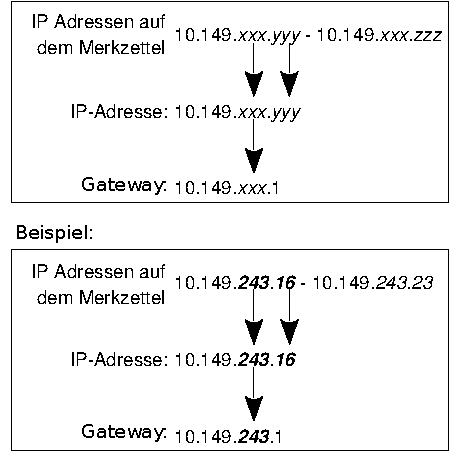
\includegraphics[width=0.4\linewidth,keepaspectratio]{Bilder/IP_Gerneric}
\end{center}
\end{minipage}

\newpage

\section{Konfiguration IP-Einstellungen}
\label{sec:network_address}
Hier sind die IP-Daten aus dem vorherigen Kapitel~\ref{sec:general} notwendig.
\subsection{Router}
Die Konfiguration der IP-Adressen auf dem Router ist modellabhängig.
Auf der folgenden Seite haben wir Schlagworte gesammelt, um in der Routeranleitung die richtigen Abschnitte zu finden.

\url{https://stustanet.de/de/support/router_instructions/}

Eine generelle Anleitung zur Verbindung des Computers mit dem Router ist in der Anleitung des Routerherstellers zu finden.

Bei Benutzung eines Routers ist es nicht notwendig, die IP-Adressen auch auf den Endgeräten (Computer, Handy, ....) einzurichten wie es im Rest von Kapitel~\ref{sec:network_address} beschrieben ist, sondern nur auf dem Router.
Bei Nicht-Mitglieder ist die Proxykonfiguration auf allen Endgeräten (Computer, Handy, ...) außer des Routers trotzdem notwendig.

\subsection{Konfiguration mit LAN-Kabel direkt am Computer (nur ohne Router notwendig)}
\subsubsection*{IP-Einstellungen LAN für Windows 10}
\begin{minipage}{0.57\textwidth}
\begin{enumerate}
	\item Klicke auf das Windowssymbol in der unteren linken Ecke und anschließend auf \textit{Einstellungen}
	\item Klicke auf \textit{Netzwerk- und Internet}.
	Scrolle nach unten bis \textit{Netzwerk- und Freigabecenter} und klicke auf diesen Punkt. Wähle in der linken Spalte den Punkt \textit{Adaptereinstellungen ändern} aus.
	Man kann auch in der Suchzeile rechts oben nach \glqq Adaptereinstellungen ändern\grqq suchen.
    \item Es sollten nun mehrere Netzwerkverbindungen aufgelistet sein. Klicke mit der \textbf{rechten} Maustaste auf \textit{Ethernet} und klicke auf \textit{Eigenschaften}.
    \item Markiere den Eintrag \textit{Internetprotokoll Version 4 (TCP/IPv4)} und klicke danach auf Eigenschaften.
    \item Jetzt gebe
    \begin{itemize}
    	\item IP-Adresse
    	\item Subnetzmaske
    	\item (Standart-)Gateway
    	\item Bevorzugter DNS-Server
    	\item Alternativer DNS-Server
    \end{itemize}
	ein.
    \item Klicke auf \textit{Erweitert} und wählen im folgenden Dialog den Reiter \textit{DNS} aus. Trage im Feld \textit{DNS-Suffix} für diese Verbindung die Suchdomäne ein.
    \item Bestätige mit \textit{OK}.
\end{enumerate}
\end{minipage}
\hfill
\begin{minipage}{0.4\textwidth}
	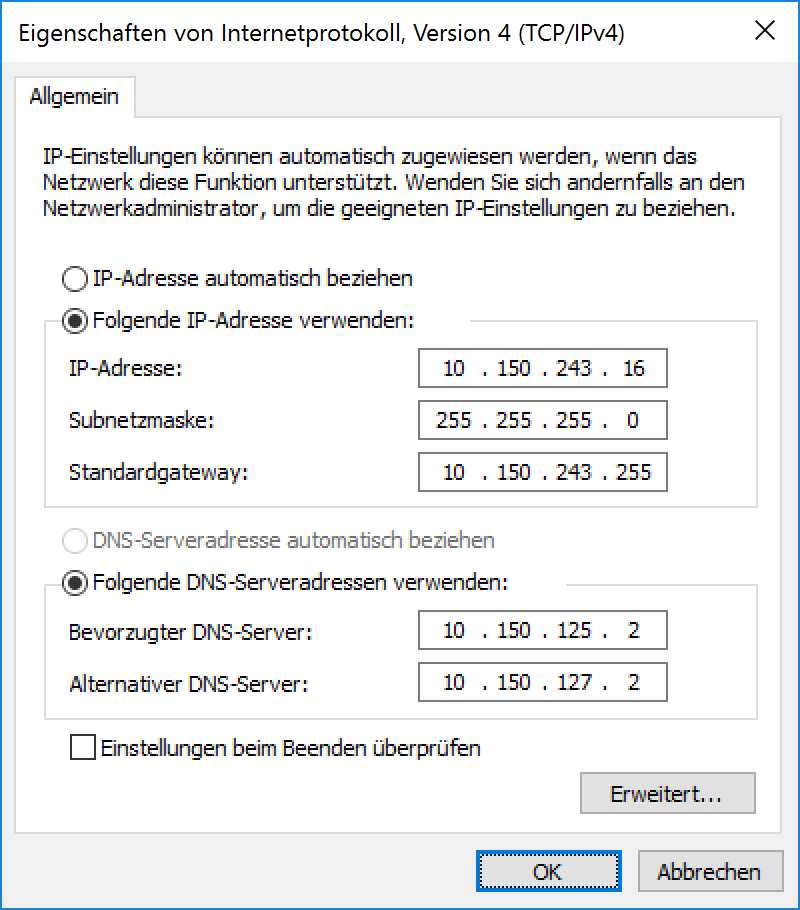
\includegraphics[width=\textwidth]{Bilder/IP_Windows}
	%  \caption{Bildunterschrift}
\end{minipage}%

\subsubsection*{IP-Einstellungen LAN für Windows 11}
\begin{minipage}{0.57\textwidth}
\begin{enumerate}
	\item Gehe in den rechts orange markierten Feldern zu \textit{Einstellungen} $\rightarrow$ \textit{Netzwerk und Internet} $\rightarrow$ \textit{Ethernet} $\rightarrow$ Bei \textit{IP-Zuweisung} klicke \textit{Bearbeiten}.
	\item Ändere das Dropdown-Menü zu \textit{Manuell}.
	\item Setze die Checkbox \textit{IPv4} auf \textit{Ein}.
	\item Jetzt trage in die rechts blau markierten Felder
		\begin{itemize}
			\item IP-Adresse
			\item Subnetzmaske
			\item Gateway
			\item Bevorzugter DNS
			\item Alternativer DNS
		\end{itemize}
	deines Zimmers von Punkt~\ref{ip_sheet} ein.
	\item Bestätige mit \textit{Speichern}.
\end{enumerate}
\end{minipage}
\hfill
\begin{minipage}{0.4\textwidth}
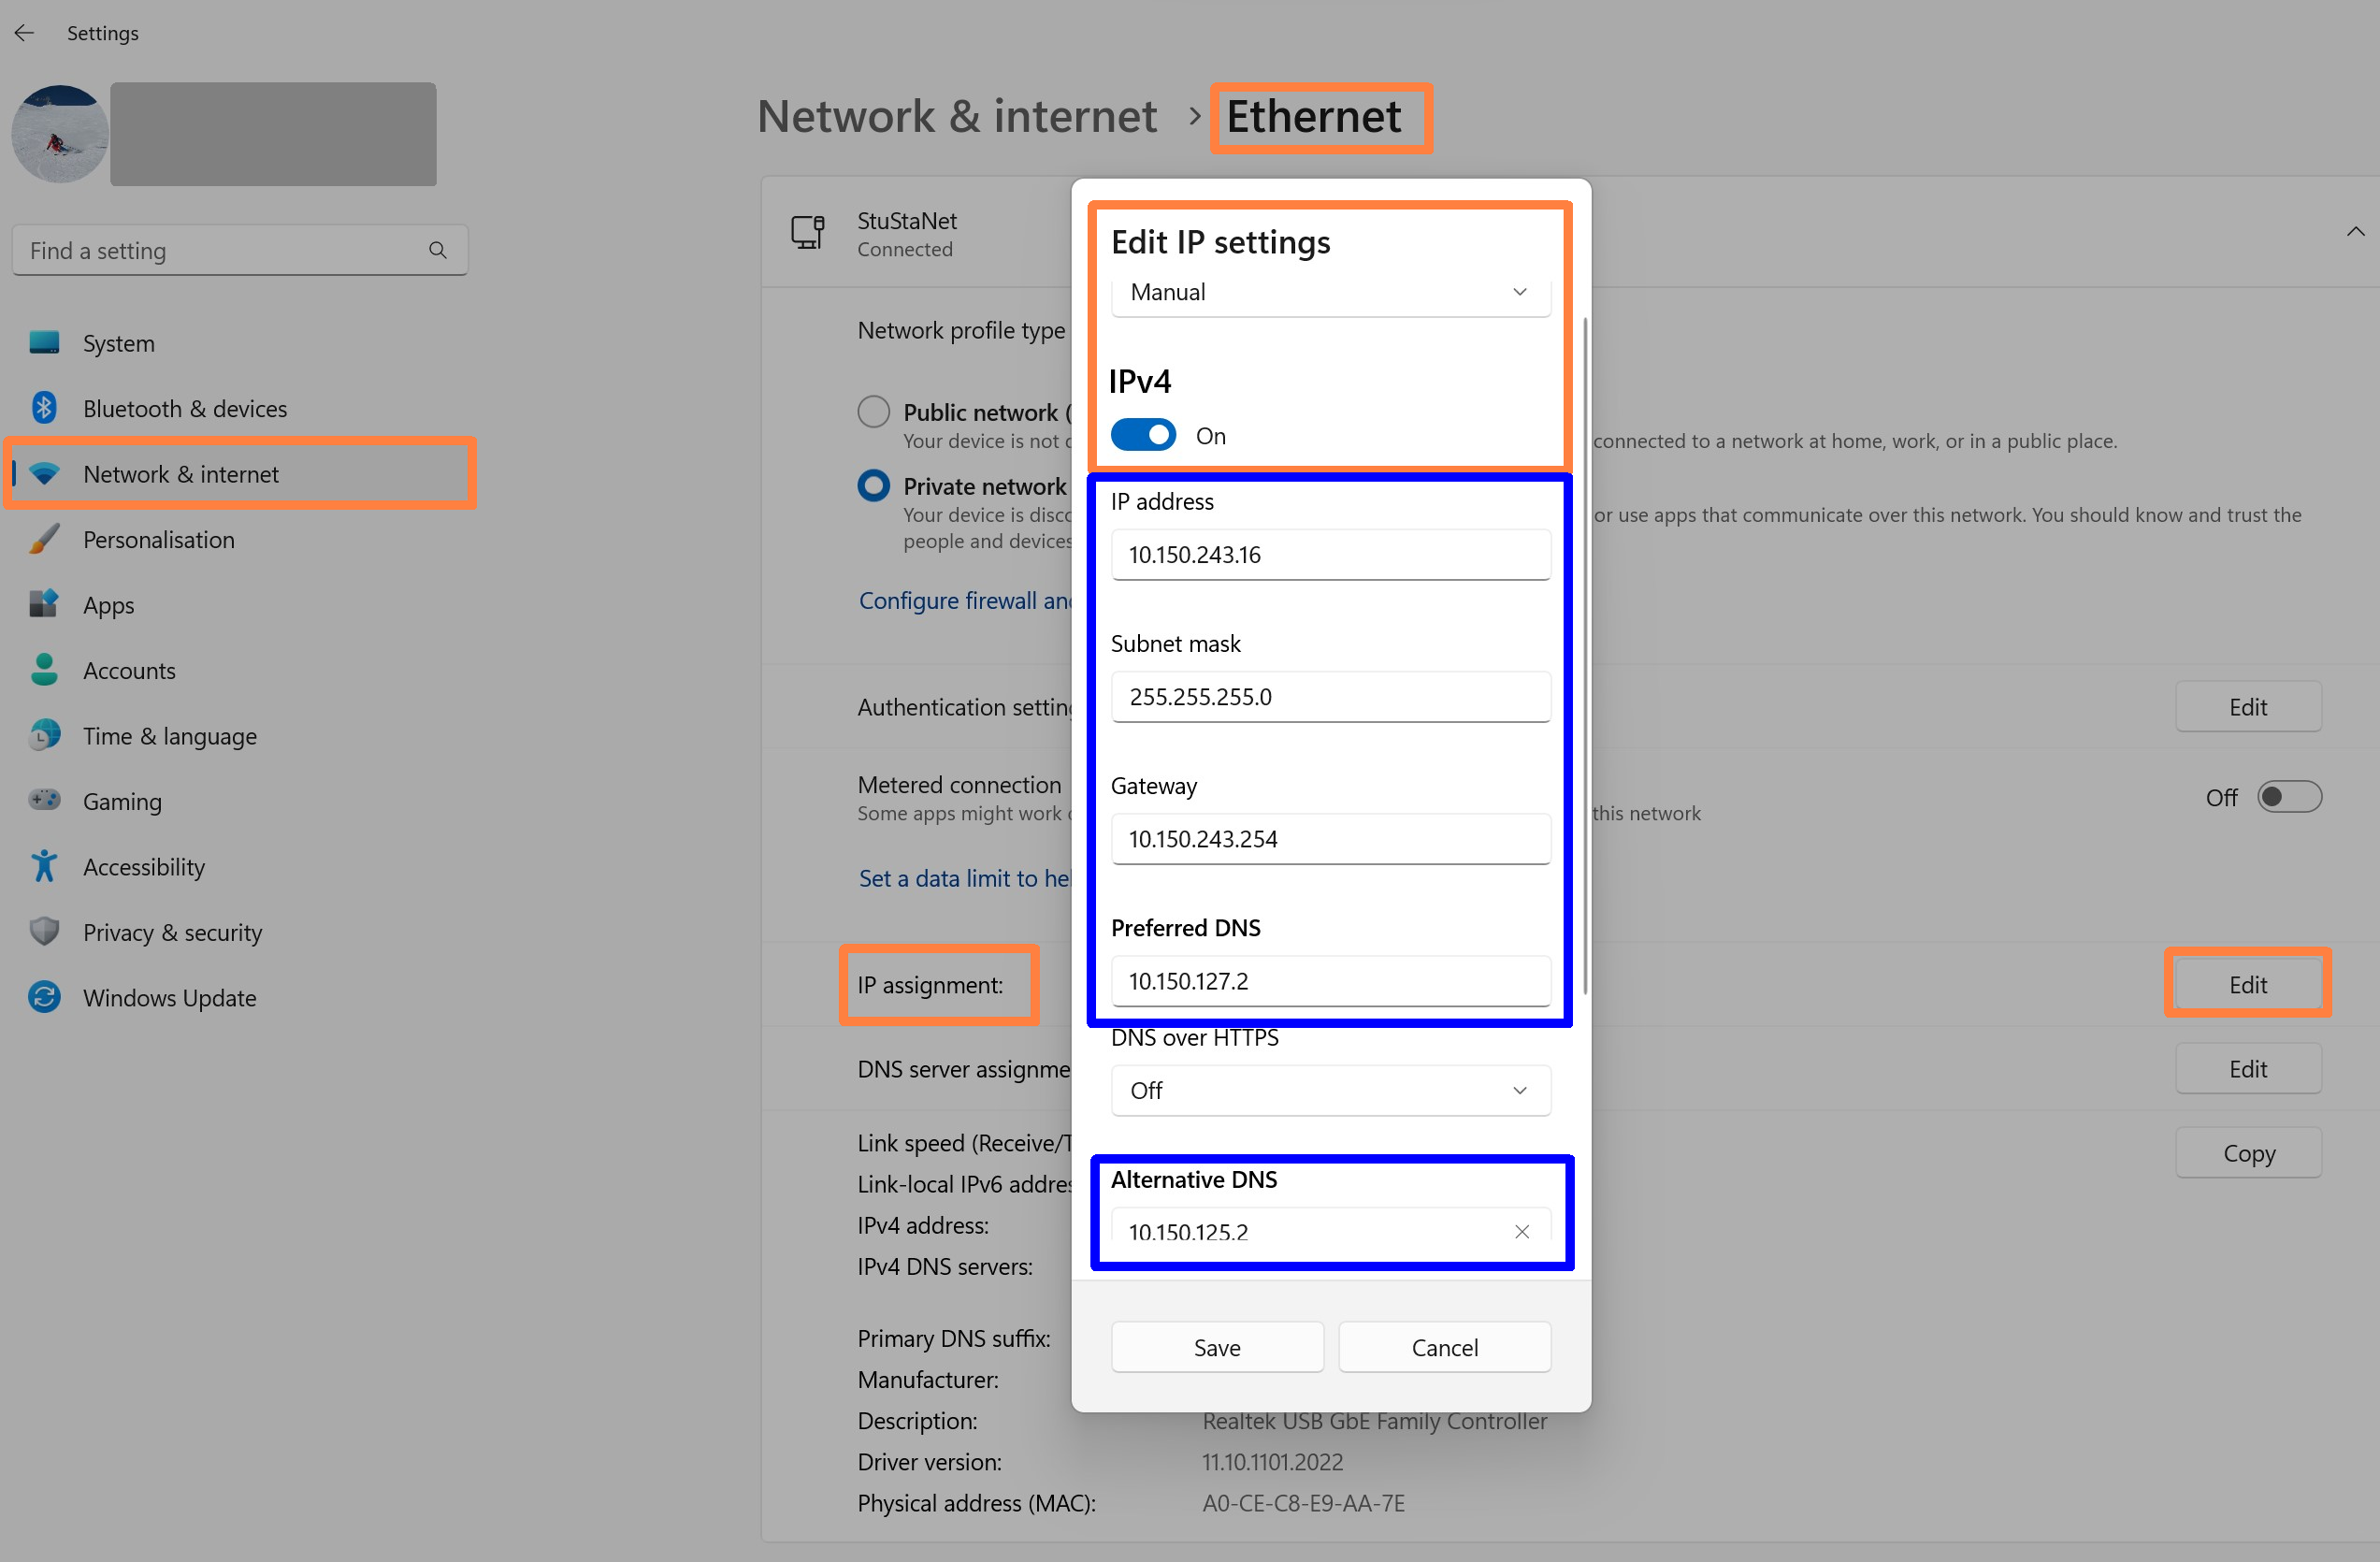
\includegraphics[width=\linewidth]{Bilder/Win11/IP_win11}
Auswählen: \textit{orange}, Ausfüllen: \textit{blau}
\end{minipage}

\subsubsection*{IP-Einstellungen LAN für Linux}

Beispiel für \textit{Networkmanager}.
Kann abweichen je nach Distribution, sollte aber im Kern ähnlich sein.

\begin{minipage}{0.57\textwidth}
\begin{enumerate}
	\item Öffne die Netzwerkkonfiguration durch Klick auf \textit{System} $\rightarrow$ \textit{Einstellungen} $\rightarrow$ \textit{Netzwerkkonfiguration}.
	\item Markiere nun im Reiter Kabelgebunden den entsprechenden Eintrag Ihrer Netzwerkkarte (im Normalfall \textit{eth0}) und klicken Sie auf den Button \textit{Bearbeiten}.
	\item Gehe zum Reiter \textit{IPv4-Einstellungen} und setze \textit{Methode} auf \textit{Manuell}.
	\item Unter \textit{Adressen} klicke auf den Button \textit{Hinzufügen}.
	\item Jetzt gebe
	\begin{itemize}
		\item IP-Adresse
		\item Subnetzmaske
		\item Gateway
		\item DNS
		\item Suchdomäne
	\end{itemize}
	ein.
	\item Bestätige mit \textit{OK} und schließe das Fenster für die Netzwerkeinstellungen.
\end{enumerate}
\end{minipage}
\hfill
\begin{minipage}{0.4\textwidth}
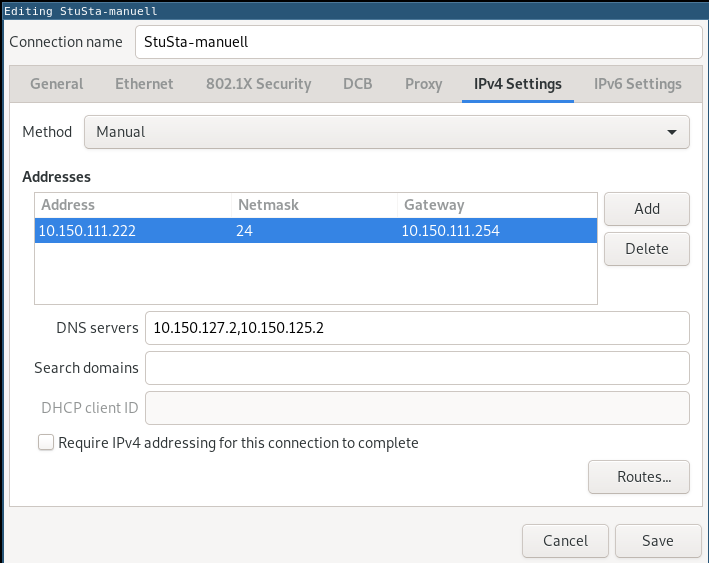
\includegraphics[width=\linewidth]{Bilder/IP_Ubuntu_neu}
\end{minipage}

\subsubsection*{IP-Einstellungen LAN ab MacOS 13.0 (Ventura)}

\begin{minipage}{0.57\textwidth}
	\begin{enumerate}
		\item Öffne die Netzwerkkonfiguration durch Klick auf \textit{Apfel} (oben links) und wählen dann \textit{Systemeinstellungen} $\rightarrow$ \textit{Netzwerk} aus.
		\item Wähle nun ihren LAN-Adapter bzw. Dock in der Liste aus.
		\item Klicke auf \textit{Details}.
		\item Gehe auf den Reiter \textit{TCP/IP}.
		\item Wähle beim Feld \textit{IPv4 Konfigurieren} die Option \textit{Manuell}.
		\item Jetzt gebe
		\begin{itemize}
			\item IP-Adresse
			\item Netzmaske/Teilnetzmaske
			\item Gateway/Router
		\end{itemize}
		ein.
		\item Als Nächstes wähle den Reiter \textit{DNS} aus.
		\item Füge beim \textit{DNS-Server} jeweils einzeln mittels \textbf{+} die beiden \textit{DNS-Server} hinzu.
		\item Füge bei \textit{Suchdomäne} mittels \textbf{+} die \textit{Suchdomäne} hinzu.
		\item Bestätige mit \textit{OK}.
	\end{enumerate}
\end{minipage}
\hfill
\begin{minipage}{0.4\textwidth}
	\centering
	\includegraphics[width=\linewidth,keepaspectratio]{Bilder/macos/ip_macos13}
	Auswählen: \textit{orange}, Ausfüllen: \textit{blau}
\end{minipage}

\subsubsection*{IP-Einstellungen LAN für MacOS (alt)}

\begin{minipage}{0.57\textwidth}
\begin{enumerate}
    \item Öffne die Netzwerkkonfiguration durch Klick auf \textit{Apfel} (oben links) und wählen dann \textit{Systemeinstellungen} $\rightarrow$ \textit{Netzwerk} aus.
    \item Markiere nun das Netzwerkgerät \textit{Ethernet}.
    \item Setze das Feld \textit{IPv4 Konfigurieren} auf \textit{Manuell}.
    \item Jetzt gebe
    \begin{itemize}
    	\item IP-Adresse
    	\item Netzmaske/Teilnetzmaske
    	\item Gateway/Router
    	\item DNS
    	\item Suchdomäne
    \end{itemize}
	in den entsprechenden Feldern ein.
	\item Bestätige mit \textit{Anwenden}.
\end{enumerate}
\end{minipage}
\hfill
\begin{minipage}{0.4\textwidth}
	\centering
	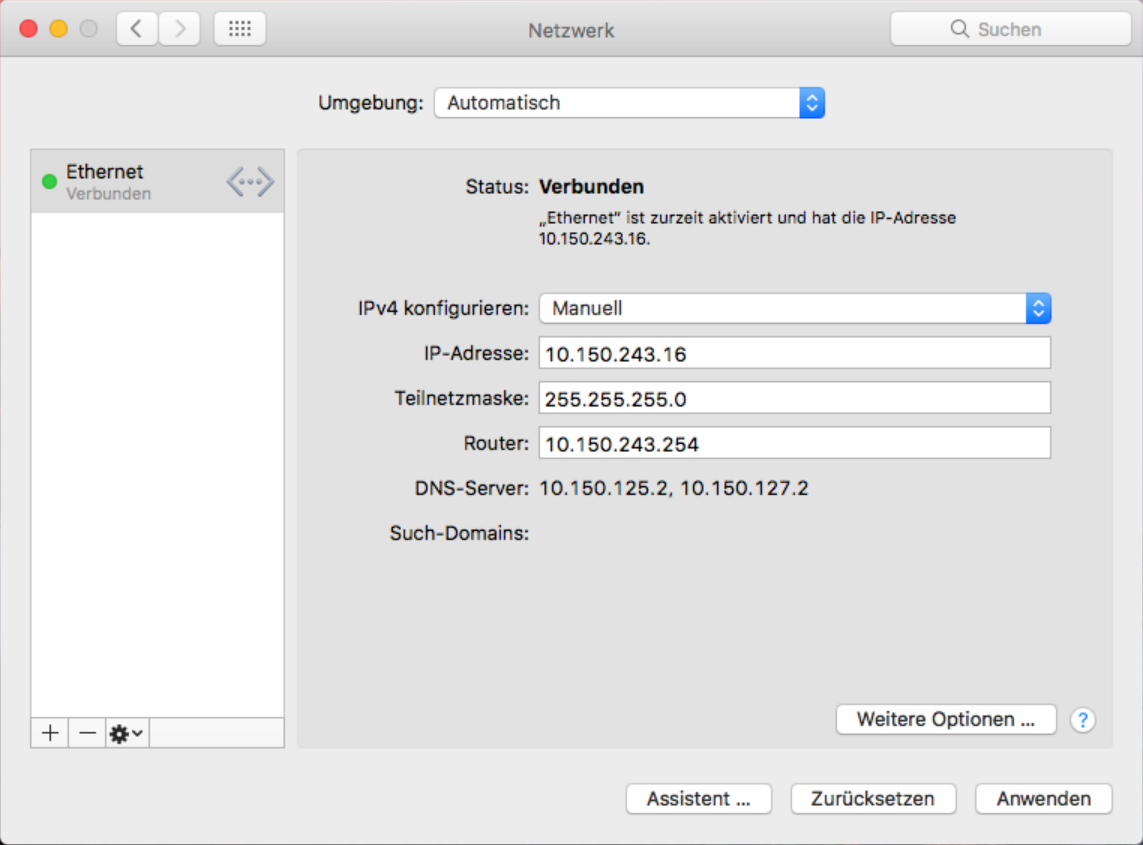
\includegraphics[width=\linewidth,keepaspectratio]{Bilder/IP_MAC}
\end{minipage}

\section{Proxyeinstellungen (nur für Nicht-Mitglieder notwendig)}
\label{sec:proxy}

\subsection*{Globaler Proxy für Windows 10/11}
\begin{enumerate}
	\item Wähle \textit{Einstellungen} $\rightarrow$ \textit{Netzwerk und Internet} $\rightarrow$ \textit{Proxy}.
	%	\item Deaktivieren Sie die Option \textit{Einstellungen automatisch erkennen}.
	\subitem \textbf{Nur Windows 11:} Klicke bei \textit{Setupskript verwenden} auf den Button  \textit{Einrichten}.
	
	\setcounter{enumi}{1}
	\item Setze \textit{Setupskript verwenden} auf \textit{Ein}.
	\item Trage als Skriptadresse die \textit{.pac Proxyskript-Adresse} des Zimmers ein.
	\item Bestätige mit \textit{Speichern}.
\end{enumerate}

\begin{figure}[h]
	\centering
	\begin{minipage}{.55\textwidth}
		\centering
		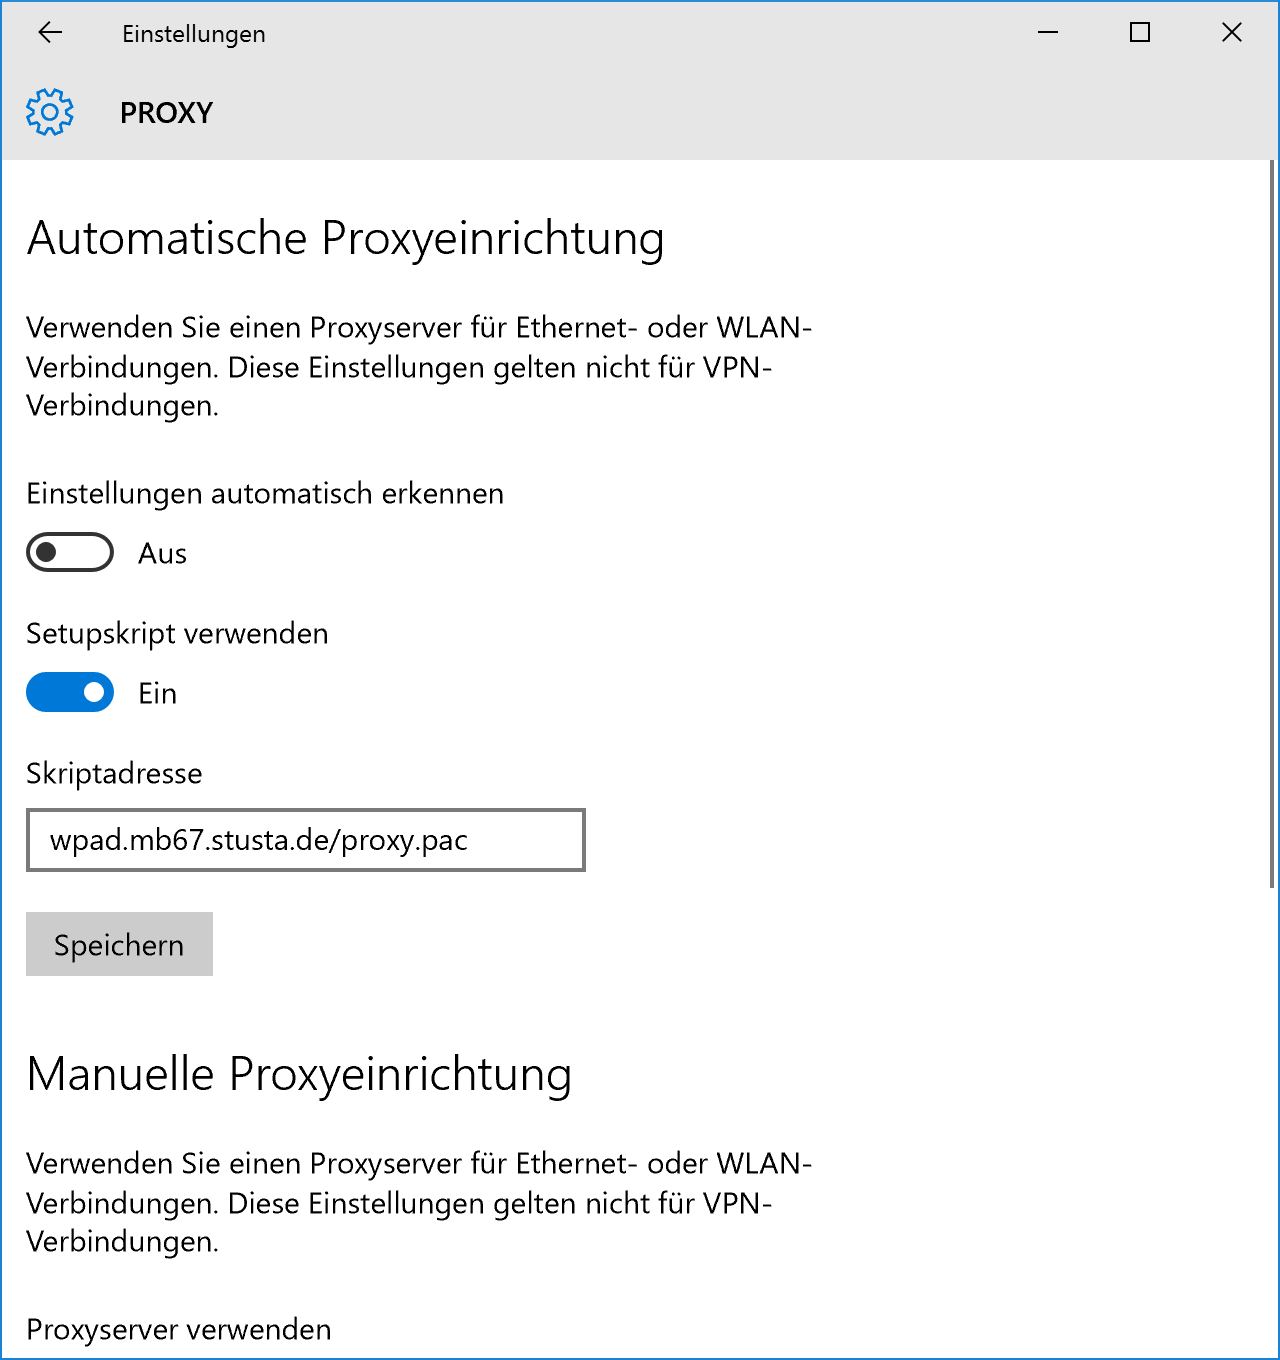
\includegraphics[height=.20\textheight]{Bilder/Proxy_Edge}
	\end{minipage}
	\begin{minipage}{.30\textwidth}
		\centering
		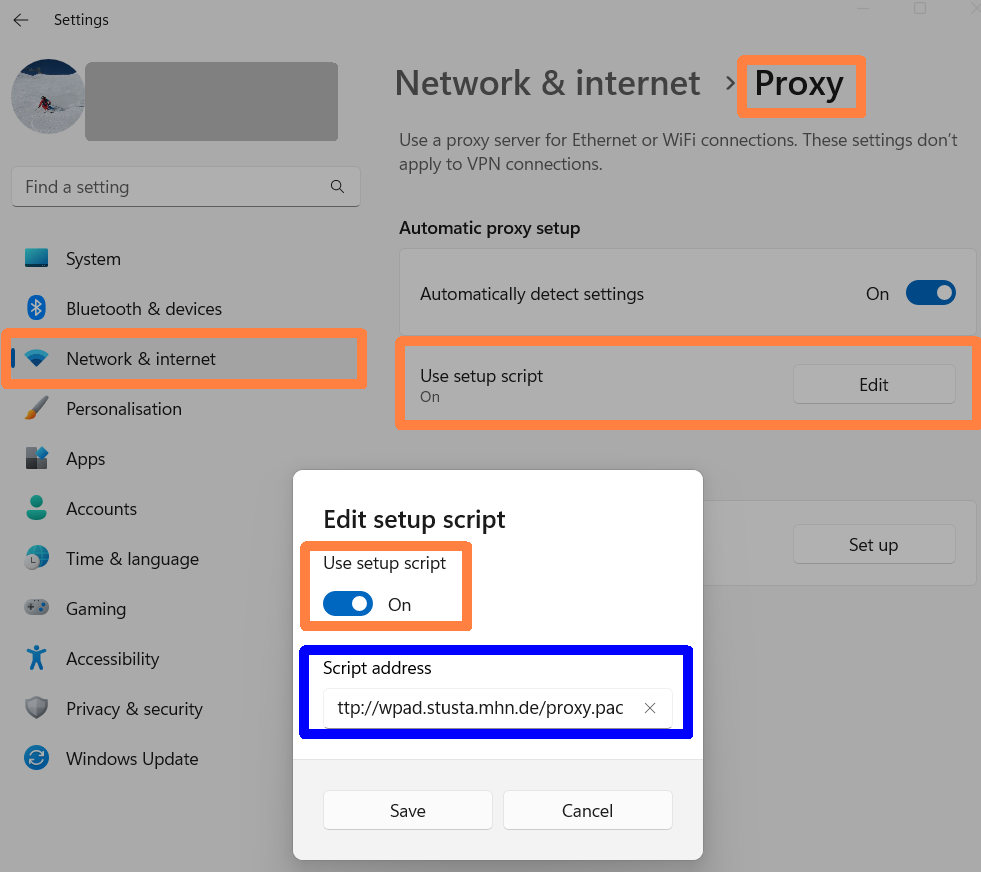
\includegraphics[height=.20\textheight]{Bilder/Win11/proxy_win11}
	\end{minipage}
\end{figure}
\begin{center}
	Links: \textit{Windows 10}, Rechts: \textit{Windows 11}
	
	Auswählen: \textit{orange}, Ausfüllen: \textit{blau}
\end{center}


\subsection*{Globaler Proxy für Linux}

Kann abweichen je nach Distribution, sollte aber im Kern ähnlich sein.
\begin{enumerate}
	\item Öffne die Netzwerk-Proxy-Einstellungen durch Klick auf \textit{System} $\rightarrow$ \textit{Einstellungen} $\rightarrow$ \textit{Netzwerk-Proxy}.
	\item Hier markiere ganz unten die Option \textit{Automatische Proxy-Konfiguration} und tragen bei URL für Auto-Konfiguration die \textit{.pac Proxyskript-Adresse} des Zimmers ein. Schließe das Fenster. 
\end{enumerate}

\subsection*{Globaler Proxy für MacOS 13.0 (Ventura)}

\begin{minipage}{0.57\textwidth}
	\begin{enumerate}
		\item Öffne die Netzwerkkonfiguration durch Klick auf \textit{Apfel} (oben links) und wählen dann \textit{Systemeinstellungen} $\rightarrow$ \textit{Netzwerk} aus.
		\item Wähle nun ihren LAN-Adapter bzw. Dock in der Liste aus.
		\item Klicke auf \textit{Details}.
		\item Gehe auf den Reiter \textit{Proxies}.
		\item Wähle \textit{Automatische Proxy-Konfiguration} aus.
		\item Gebe in \textit{URL} die \textit{.pac Proxyskript-Adresse} des Zimmers ein.
		\item Als Nächstes wähle den Reiter \textit{DNS} aus.
		\item Füge beim \textit{DNS-Server} jeweils einzeln mittels \textbf{+} die beiden \textit{DNS-Server} hinzu.
		\item Füge bei \textit{Suchdomäne} mittels \textbf{+} die \textit{Suchdomäne} hinzu.
		\item Bestätige mit \textit{OK}.
	\end{enumerate}
\end{minipage}
\hfill
\begin{minipage}{0.4\textwidth}
	\centering
	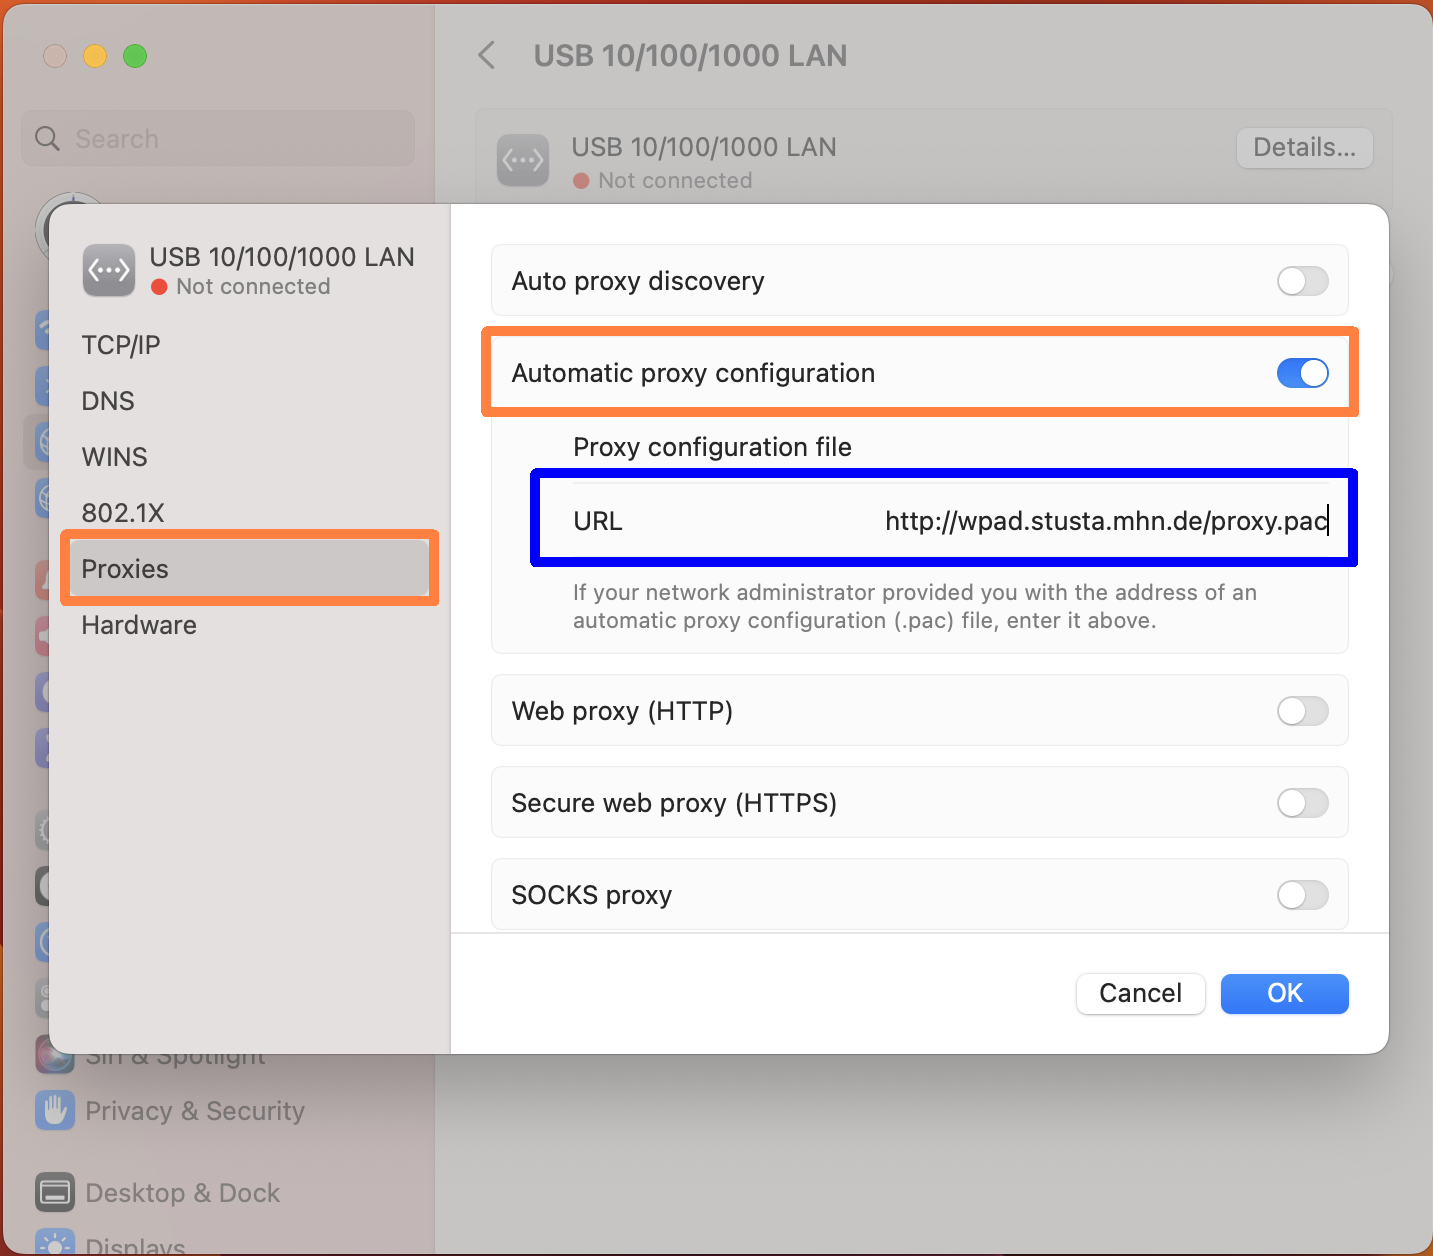
\includegraphics[width=\linewidth,keepaspectratio]{Bilder/macos/proxy_macos13}
	Auswählen: \textit{orange}, Ausfüllen: \textit{blau}
\end{minipage}

\subsection*{Globaler Proxy für MacOS (alt)}
\begin{enumerate}
	 \item Öffne die Netzwerkkonfiguration durch Klick auf \textit{Apfel} (oben links) und wählen dann \textit{Systemeinstellungen} $\rightarrow$ \textit{Netzwerk} aus.
	\item Markiere nun das Netzwerkgerät \textit{Ethernet}.
	\item Öffne mit dem Button \textit{Weitere Optionen...} die Detaileinstellungen und wechsle auf die Registerkarte \textit{Proxies}.
	\item Setze bei \textit{Zu konfigurierendes Protokoll} vor \textit{Autom. Proxy-Konfiguration} einen Haken und tragen rechts bei URL die \textit{.pac Proxyskript-Adresse} ihres Zimmers ein. Schließe die Detaileinstellungen mit \textit{OK} und bestätige erneut mit \textit{Anwenden}. Man kann die Netzwerkeinstellungen dann schließen.
\end{enumerate}

\subsection*{Globaler Proxy Android}
Bei den verschiedenen Herstellern kann das Interface leider abweichen.
Wenn du Probleme hast, kann du versuchen im Internet nach Anleitungen für dein Handymodell in Verbindung mit den Schlagworten \textit{Proxy Einrichtung} suchen.

\subsubsection*{Google Pixel Android 12}
\begin{enumerate}
	\item Öffne die WLAN-Einstellungen.
	\item Klicke auf das Zahnrad neben dem Namen deines WLAN-Netzwerkes.
	\item Klicke auf das Stiftsymbol am oberen rechten Bildschirmrand.
	\item Aktiviere das Drop-Down-Menü \textit{Erweiterte Optionen}.
	\item Wähle unter \textit{Proxy} den Punkt \textit{Automatische Proxykonfiguration}.
	\item Trage als \textit{PAC-URL} die \textit{.pac Proxyskript-Adresse} des Zimmers ein.
	\item Bestätige mit \textit{Speichern}.
\end{enumerate}

\begin{figure}[h]
	\centering
	\begin{minipage}{0.24\textwidth}
		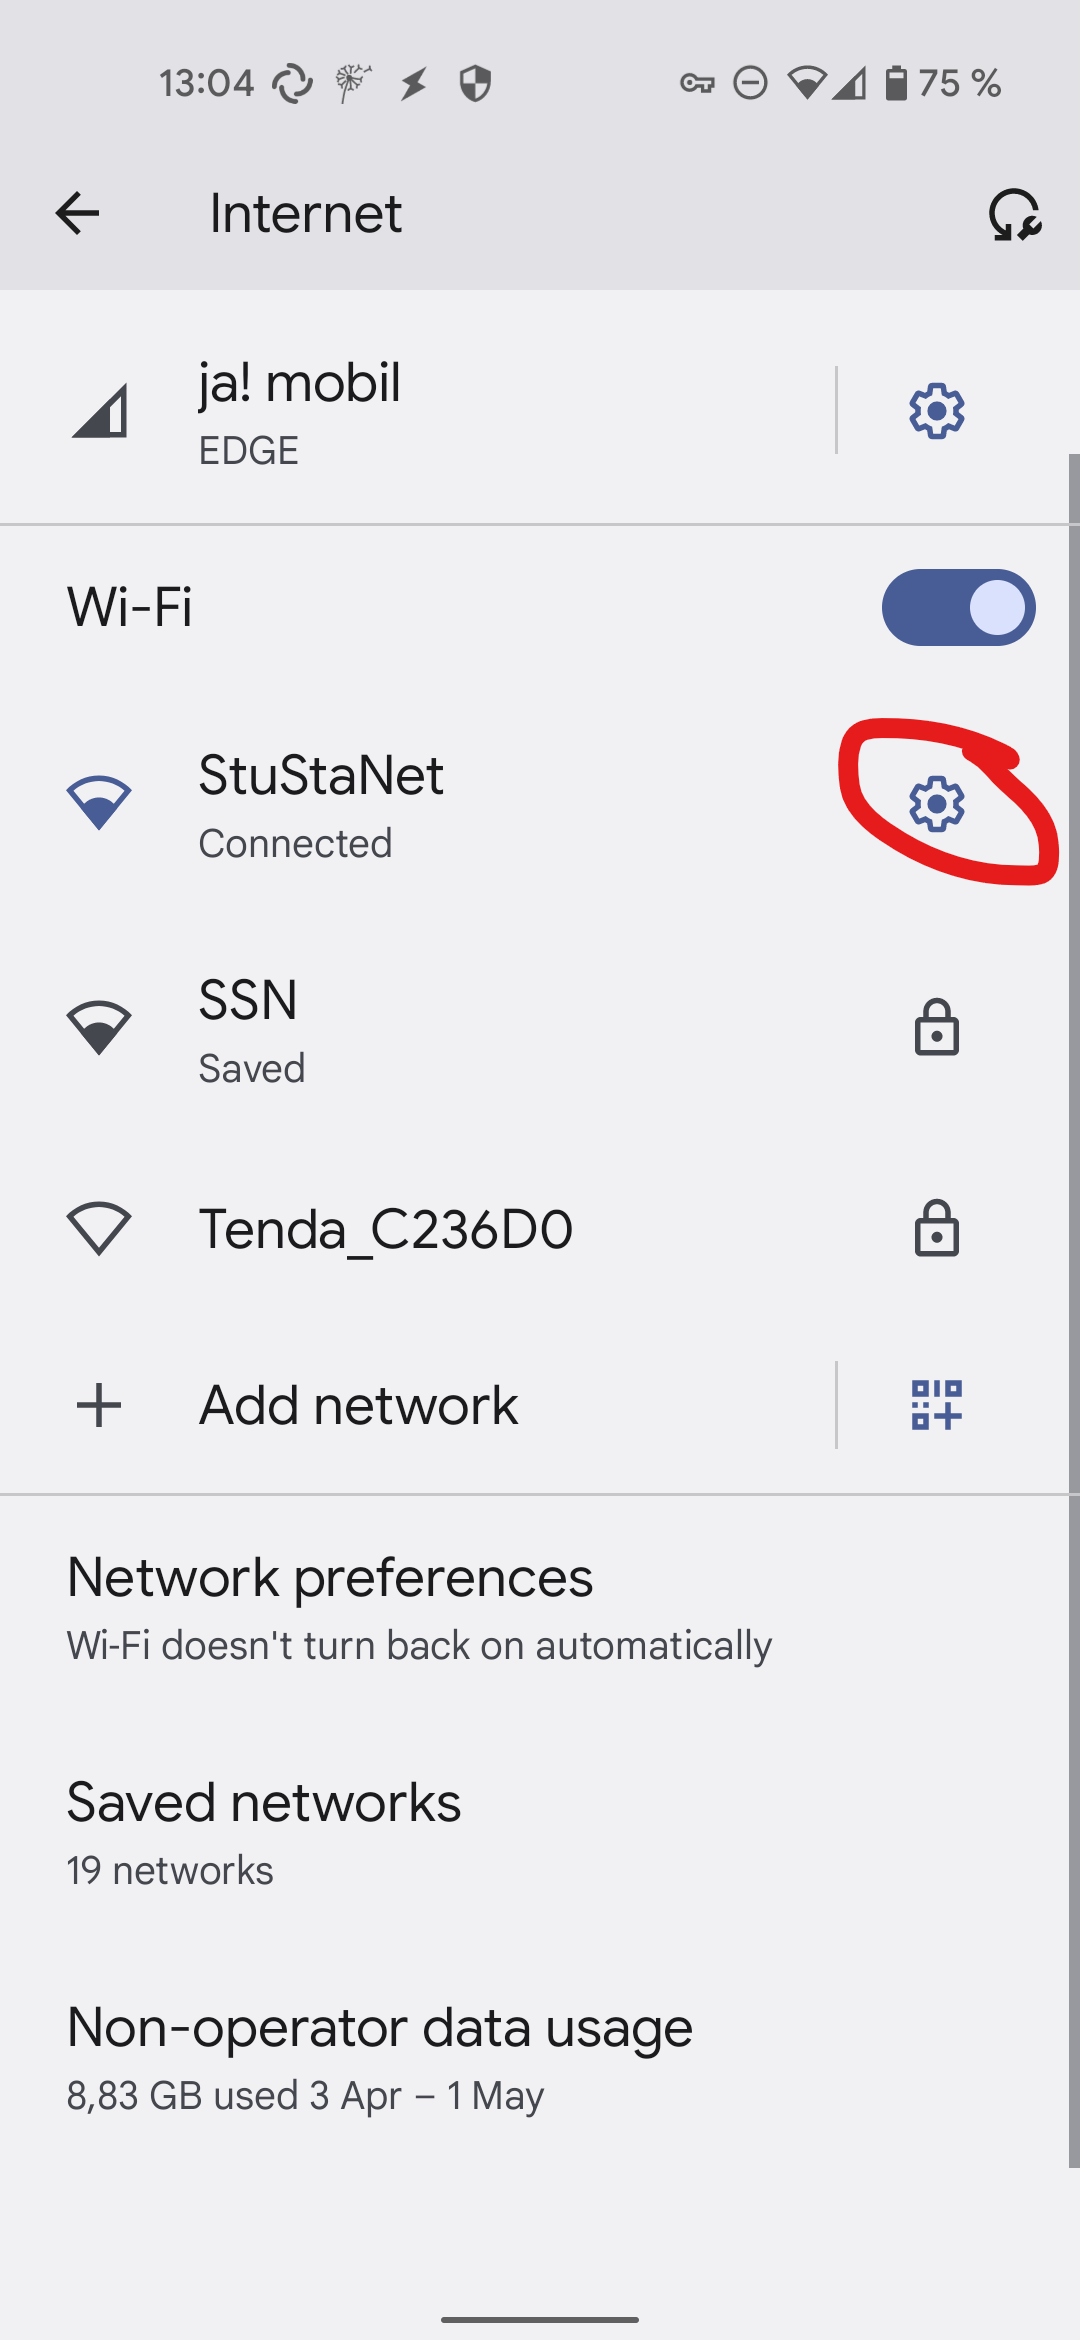
\includegraphics[width=0.7\linewidth,keepaspectratio]{Bilder/Android/android12_1}
	\end{minipage}
	\begin{minipage}{0.24\textwidth}
		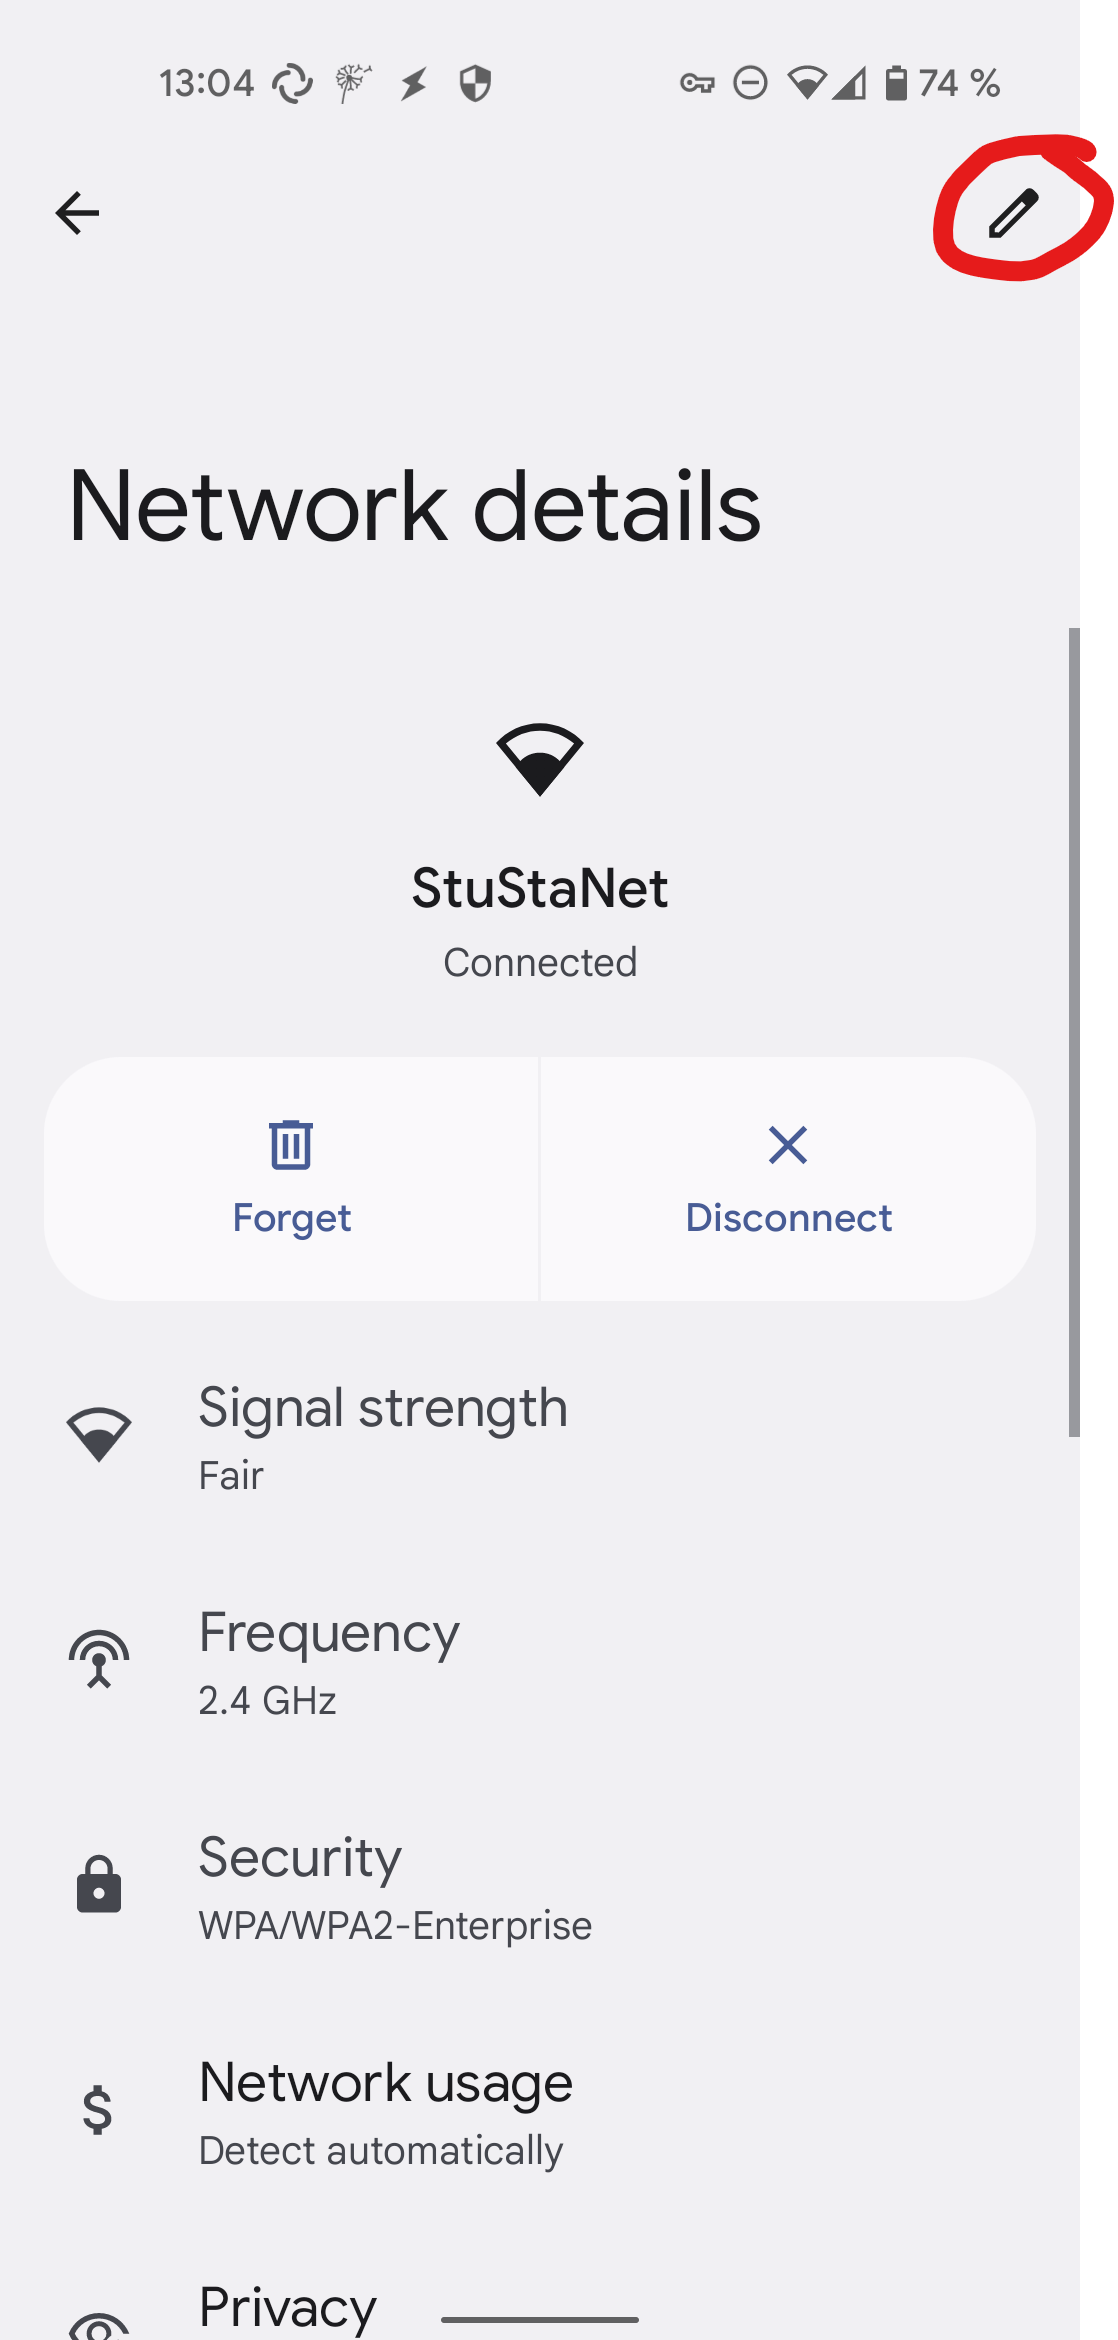
\includegraphics[width=0.7\linewidth,keepaspectratio]{Bilder/Android/android12_2}
	\end{minipage}
	\begin{minipage}{0.24\textwidth}
		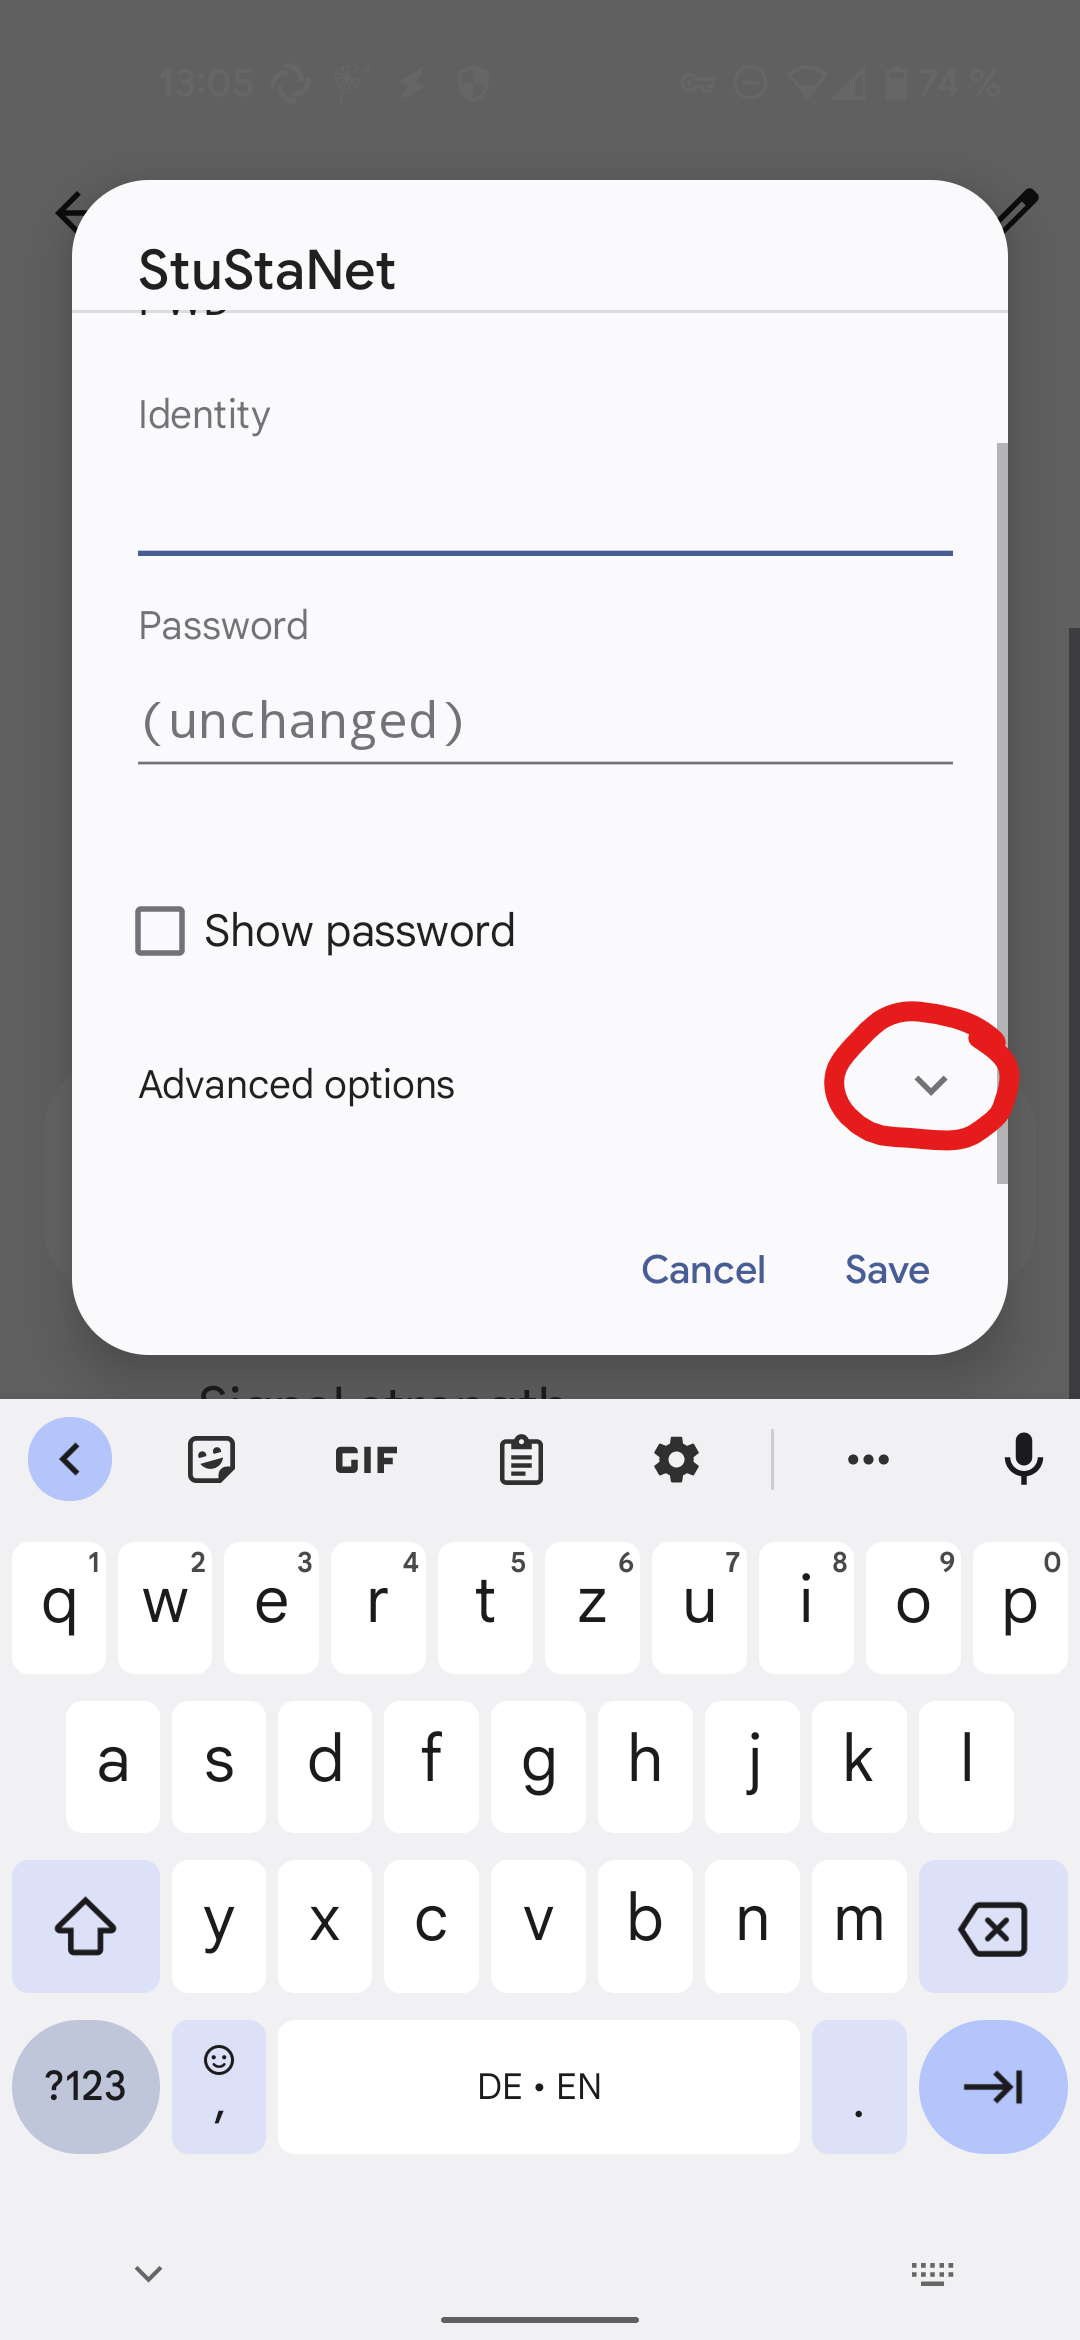
\includegraphics[width=0.7\linewidth,keepaspectratio]{Bilder/Android/android12_3}
	\end{minipage}
	\begin{minipage}{0.24\textwidth}
		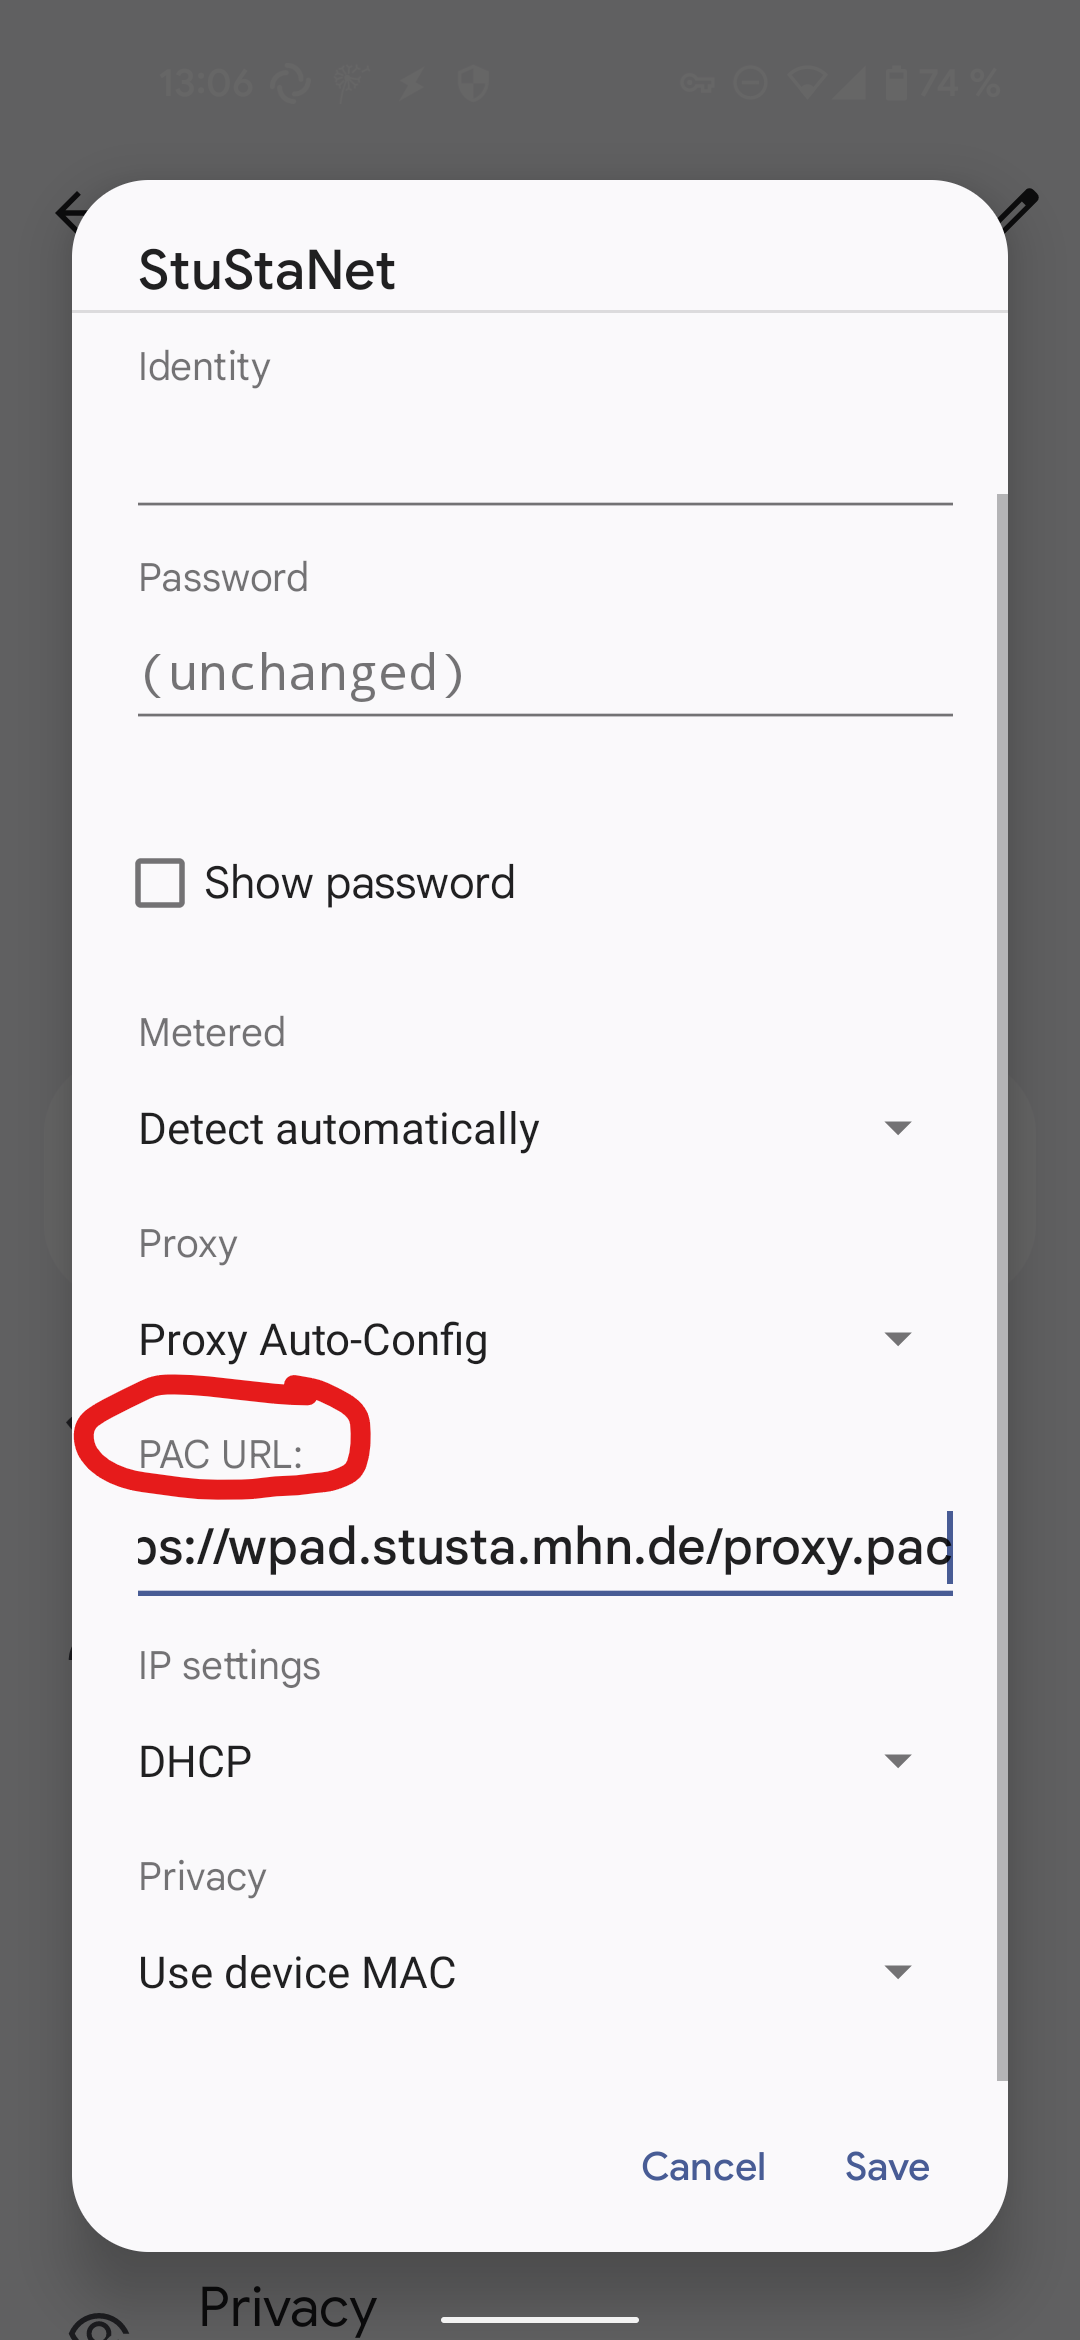
\includegraphics[width=0.7\linewidth,keepaspectratio]{Bilder/Android/android12_4}
	\end{minipage}
	Rote Markierungen folgen
\end{figure}

\subsection*{Globaler Proxy andere Geräte}
Wenn du Probleme hast, kann du versuchen im Internet nach Anleitungen für dein Gerät in Verbindung mit den Schlagworten \textit{Proxy Einrichtung} suchen.

\subsection*{Browser}
Die meisten Browser wie Chrome, Firefox und Edge nutzen mittlerweile standardmäßig den Proxy des Betriebssystems wie in Kapitel~\ref{sec:proxy} eingerichtet.

Somit ist eine getrennte Konfiguration nicht notwendig

\section{Kontrolle \& Debugging}
\label{sec:debugging}
Zur Kontrolle kann man versuchen aus dem Zimmeranschluss (nicht Handynetz!) die folgenden Seiten aufzurufen.
\begin{itemize}
	\item \url{http://selftest.stustanet.de}
	\begin{itemize}
		\item Rudimentäre Selbstdiagnose
	\end{itemize}
	\item \url{https://wiki.stusta.de}
	\begin{itemize}
		\item StuSta-Internes Wiki
		\item Bei Fehler Hinweis auf Problem bei IP-Konfiguration aus Kapitel~\ref{sec:network_address} oder dem Anschluss des Router/Computers aus Kapitel~\ref{sec:general}.
		\item Falls aufrufbar, aber andere Seiten nicht, Hinweis auf Probleme mit Proxykonfiguration aus Kapitel~\ref{sec:proxy}.
	\end{itemize}
\end{itemize}
Weitere Hilfen gibt es auf \mbox{\url{https://stustanet.de/de/support/}}.
\end{document}
